% !TEX root=../root.tex

We present simulation results to demonstrate the effectiveness of the proposed estimation
algorithm.
A multirotor UAV and a landing vehicle are simulated using the dynamics presented
in~\eqref{eq:uav_dynamics} and~\eqref{eq:goal_dynamics}.
The standard deviations used for the zero-mean
Guassian noise processes in the dynamics are found
in~\tabref{tab:sim_process_noises}.
As the estimator depends on
tracking and estimating the positions of visual features that are rigidly
attached to the landing vehicle, feature positions on the landing vehicle
are also simulated.
Positions for each feature in the goal frame are
randomly sampled from the
uniform distribution
\begin{equation}
  \vect{r}_{i/g}^g = \mathcal{U}
  \left[ \begin{bmatrix} -2 \\ -2 \\ -1 \end{bmatrix},
  \begin{bmatrix} 2 \\ 2 \\ 1 \end{bmatrix} \right].
  \label{eq:uniform_dist}
\end{equation}
At each time step of the simulation, features are given a one percent chance
of disappearing. When a feature disappears, a new feature is randomly
generated by sampling from~\eqref{eq:uniform_dist}.

The sensor measurements that are provided to the estimator are simulated using the true
state of the simulation. These sensor measurements include accelerometer,
gyroscope, global position of the UAV, global attitude 
of the UAV, relative position and attitude from the fiducial landing marker, and
feature locations in the camera frame. All measurements are
corrupted with white Gaussian noise. The sensor noise parameters along with the
rate at which each sensor is sampled are found
in~\tabref{tab:sim_meas_noise}.

The landing vehicle was initialized with initial conditions given by
\begin{equation}
  \begin{bmatrix}
    v_x \\
    v_y \\
    \theta_I^g \\
    \omega
  \end{bmatrix}
  =
  \begin{bmatrix}
    0.5 \hphantom{\cdot} m/s \\
    0 \hphantom{\cdot} m/s \\
    1.5 \hphantom{\cdot} rad \\
    0.5 \hphantom{\cdot} rad/s
  \end{bmatrix}
\end{equation}
The 
simulated camera was oriented at a yaw angle of $\pi/2 \hphantom{\cdot} rad$ with respect to the body
frame and $p_{c/b}^b = \begin{bmatrix}0.25, & -0.2, &
0.4 \end{bmatrix}^\transpose m$.

The simulation results for a 30 second simulation in which the estimator does
not use any visual features are seen in
Figures~\ref{fig:no_lms_gp}, \ref{fig:no_lms_gv}, \ref{fig:no_lms_gatt}. In the
experiment shown, the measurements from the fiducial landing marker are not used
after $t = 5 \hphantom{\cdot} s$ to demonstrate the performance of the proposed
estimation algorithm when the fiducial marker is not detected for significant
periods of time. The figures clearly show that when measurements from the
fiducial marker are not available, the covariance of the estimate grows rapidly
and the estimated state of the landing vehicle quickly becomes inaccurate. This
matches our intuition as the estimator receives no information about the landing
vehicle after $t = 5 \hphantom{\cdot} s$ and therefore is only able to propagate
the dynamics of the system. We note that the $z$ direction of the estimated
relative goal position is the exception as the landing vehicle is constrained to
move only in the $xy$ plane. We do not include the plots of the UAV states,
$\vect{x}_{\text{UAV}}$, as it is well known that these states are easily
estimated with the given measurements.

Simulation results for the same scenario, but in which the estimator uses a
maximum of 10 visual features, are seen in
Figures~\ref{fig:with_lms_gp}, \ref{fig:with_lms_gv}, \ref{fig:with_lms_gatt}.
These figures clearly show that even after $t = 5 \hphantom{\cdot} s$ when the
fiducial marker measurements are no longer available, the estimated states of
the landing vehicle remain accurate with relatively tight covariance bounds. We
reiterate that the only information the estimator receives during this time is
the measured pixel locations of unknown visual features on the landing vehicle.

To further demonstrate performance, 100 simulation runs of the same scenario
mentioned above were performed
both using ten visual features and using zero visual features. The L2 norm of
the $xy$ error of the estimated goal position state are plotted
with respect to time in
Figures~\ref{fig:mc_no_lms_xy_err}~and~\ref{fig:mc_with_lms_xy_err}. While the
error when using 10 features
almost entirely remains under 1 $m$ for all 100 simulations, the error when using
no features quickly grows very large, reaching an error of over 10 $m$ in many
of the runs.

\begin{table}[h!]
  \begin{center}
    \caption{Simulation Motion Model Parameters.}
    \label{tab:sim_process_noises}
    \begin{tabular}{l|l}
      \textbf{Parameter} & \textbf{Std. Deviation} \\
      \hline
      $\vect{\eta}_{\beta_a}$ & 0.05 $m/s^2$ \\
      $\vect{\eta}_{\beta_\omega}$ & 0.01 $rad/s$ \\
      $\vect{\eta}_{gv}$ & 5 m/s \\
      $\vect{\eta}_{g\omega}$ & 5 rad/s \\
      % v & 5 m/s \\
      % landmark $x_{\text{min}}$ & -2 m \\
      % landmark $x_{\text{max}}$ & 2 m \\
      % landmark $y_{\text{min}}$ & -2 m \\
      % landmark $y_{\text{max}}$ & 2 m \\
      % landmark $z_{\text{min}}$ & -1 m \\
      % landmark $z_{\text{max}}$ & 1 m \\
      % landmark disappear prob. & 1\% \\
    \end{tabular}
  \end{center}
\end{table}

\begin{table}[h!]
  \begin{center}
    \caption{Simulation Sensor Noise Characteristics.}
    \label{tab:sim_meas_noise}
    \begin{tabular}{l|l|l}
      \textbf{Measurement} & \textbf{Std Dev} & \textbf{Rate} \\
      \hline
      Accelerometer & 0.2 $m/s^2$ & 250 Hz \\
      % walk & 0.05 $m/s^2$  \\
      % init & 0.01 $m/s^2$ \\
      Gyroscope & 0.1 $rad/s$ & 250 Hz \\
      % walk & 0.01 $rad/s$  \\
      % init & 0.01 $rad/s$ \\
      UAV global position & 0.1 $m$ & 10 Hz \\
      UAV global attitude & 0.1 $rad$ & 10 Hz \\
      Fiducial marker position & 0.1 $m$ & 30 Hz \\
      Fiducial marker attitude & 0.1 $rad$ & 30 Hz \\
      Visual feature image point & 2.0 pixels & 30 Hz \\
    \end{tabular}
  \end{center}
\end{table}

\begin{figure}
  \centering
  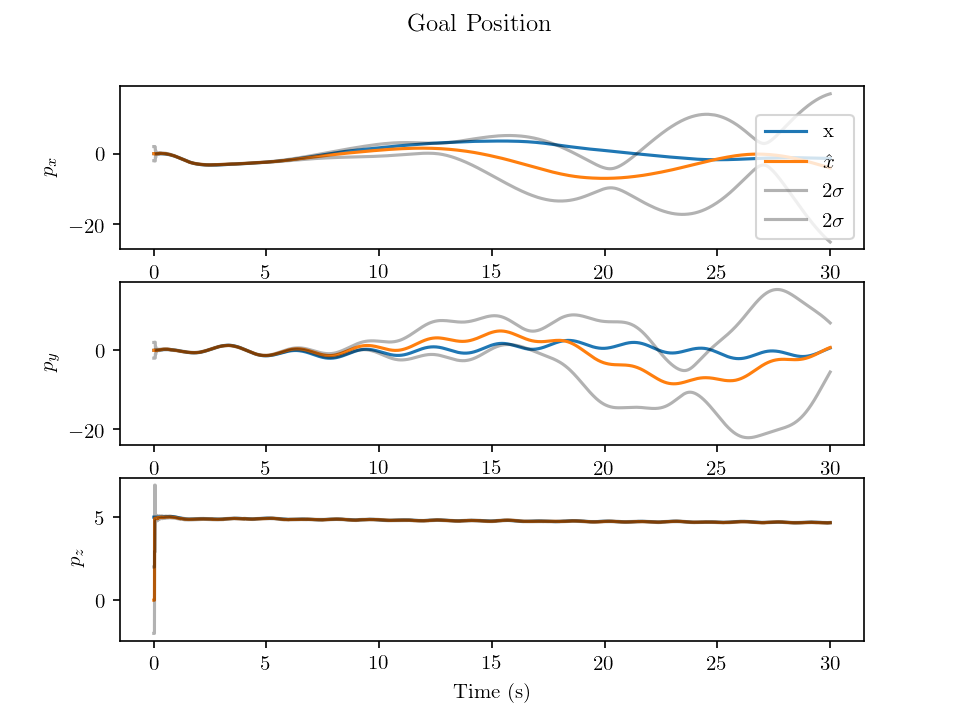
\includegraphics[scale=0.5]{plots/no_lms_gp.png}
  \caption{Simulation results with the estimator using no visual
  features. The blue line represents the true state while the orange line
  represents the estimated state. The two grey lines show a 2 $\sigma$ bound for
  the estimate based on the estimated covariance. Measurements from the fiducial
  marker are not used after $t$~=~5
$s$ to demonstrate the performance of the estimator.}
  \label{fig:no_lms_gp}
\end{figure}

\begin{figure}
  \centering
  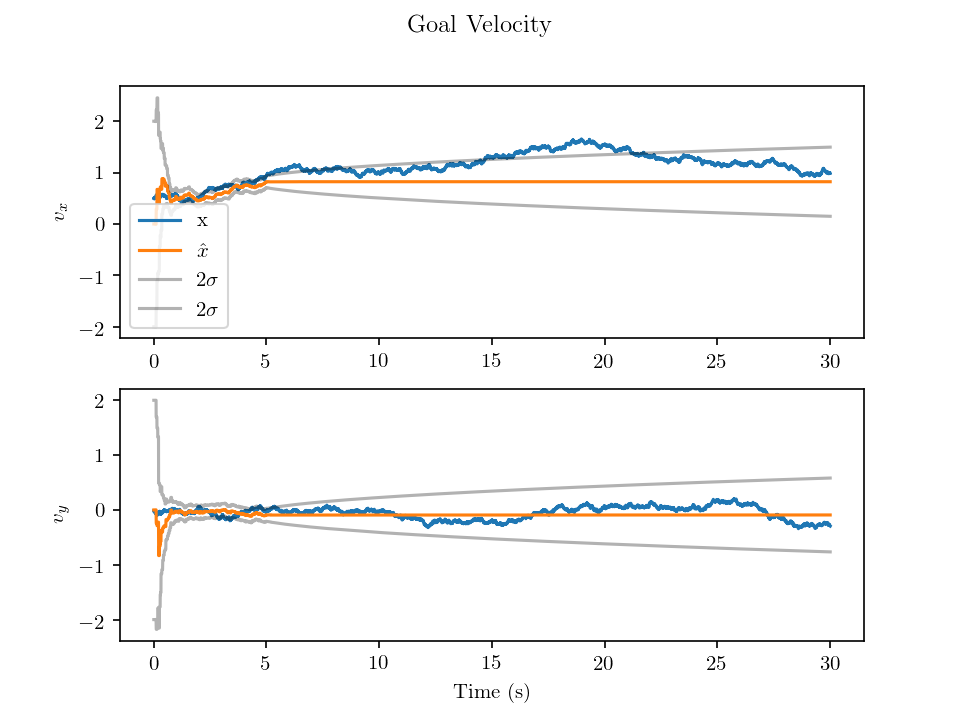
\includegraphics[scale=0.5]{plots/no_lms_gv.png}
  \caption{Simulation results with the estimator using no visual
  features. The blue line represents the true state while the orange line
  represents the estimated state. The two grey lines show a 2 $\sigma$ bound for
  the estimate based on the estimated covariance. Measurements from the fiducial
  marker are not used after $t$~=~5
$s$ to demonstrate the performance of the estimator.}
  \label{fig:no_lms_gv}
\end{figure}

\begin{figure}
  \centering
  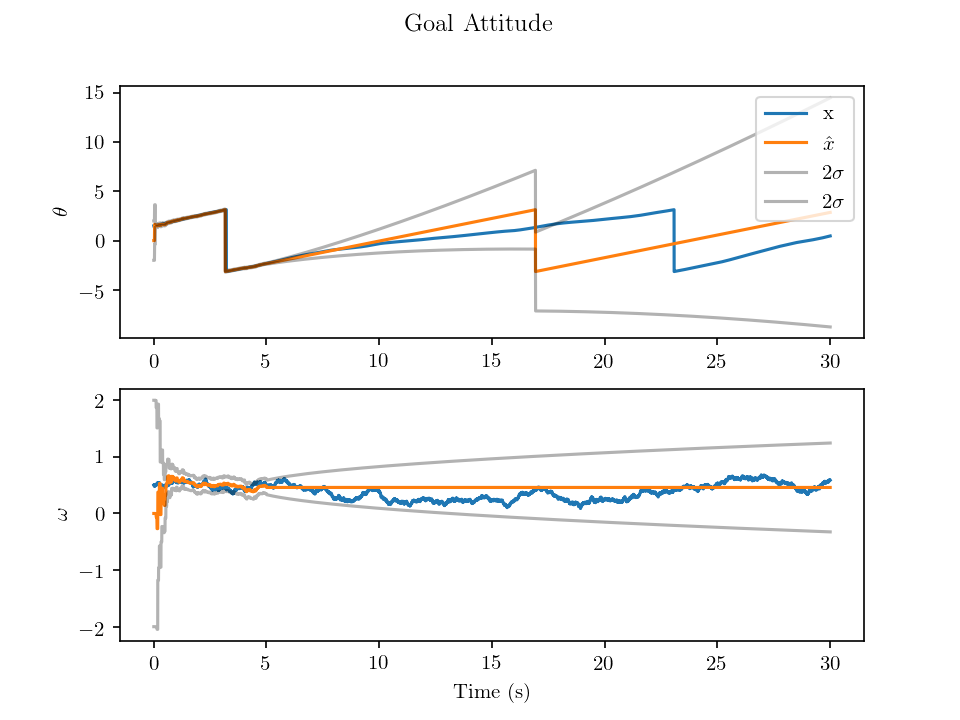
\includegraphics[scale=0.5]{plots/no_lms_gatt.png}
  \caption{Simulation results with the estimator using no visual
  features. The blue line represents the true state while the orange line
  represents the estimated state. The two grey lines show a 2 $\sigma$ bound for
  the estimate based on the estimated covariance. Measurements from the fiducial
  marker are not used after $t$~=~5
$s$ to demonstrate the performance of the estimator.}
  \label{fig:no_lms_gatt}
\end{figure}

\begin{figure}
  \centering
  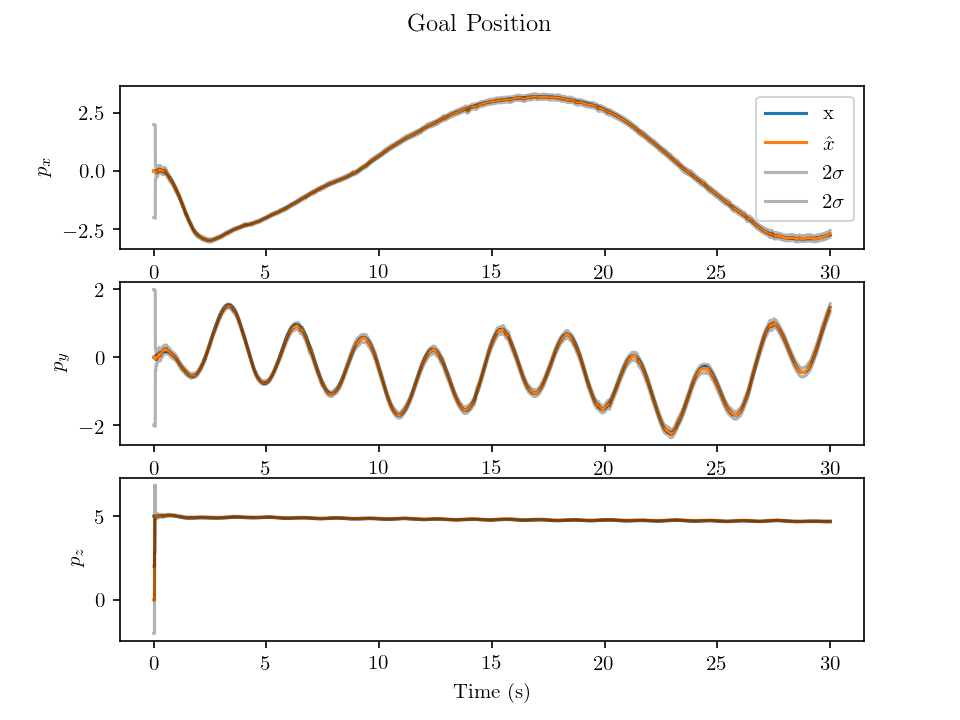
\includegraphics[scale=0.5]{plots/with_lms_gp.png}
  \caption{Simulation results with estimator using a maximum of ten visual
  features. Measurements from the fiducial marker are not used after $t$ = 5
$s$ to demonstrate the performance of the estimator.}
  \label{fig:with_lms_gp}
\end{figure}

\begin{figure}
  \centering
  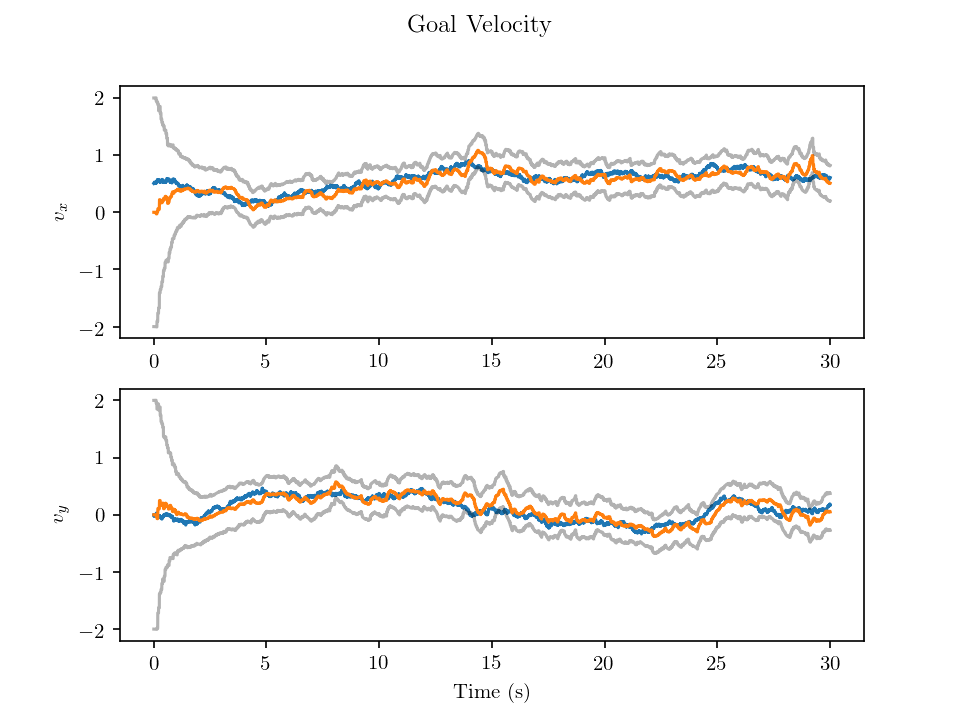
\includegraphics[scale=0.5]{plots/with_lms_gv.png}
  \caption{Simulation results with estimator using a maximum of ten visual
  features. Measurements from the fiducial marker are not used after $t$ = 5
$s$ to demonstrate the performance of the estimator.}
  \label{fig:with_lms_gv}
\end{figure}

\begin{figure}
  \centering
  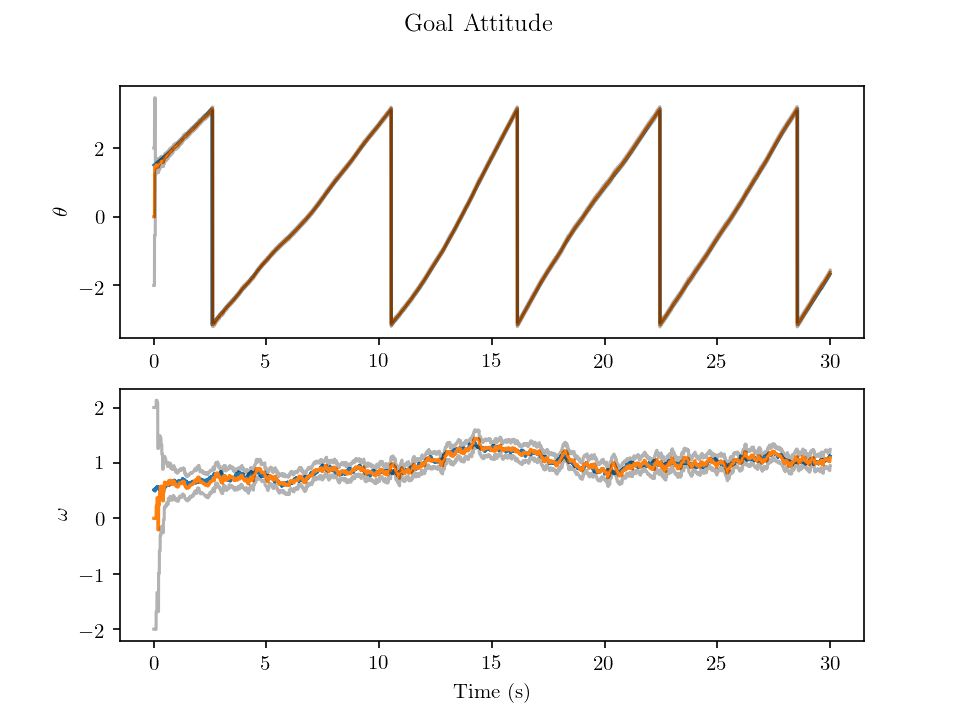
\includegraphics[scale=0.5]{plots/with_lms_gatt.png}
  \caption{Simulation results with estimator using a maximum of ten visual
  features. Measurements from the fiducial marker are not used after $t$ = 5
$s$ to demonstrate the performance of the estimator.}
  \label{fig:with_lms_gatt}
\end{figure}


\begin{figure}
  \centering
  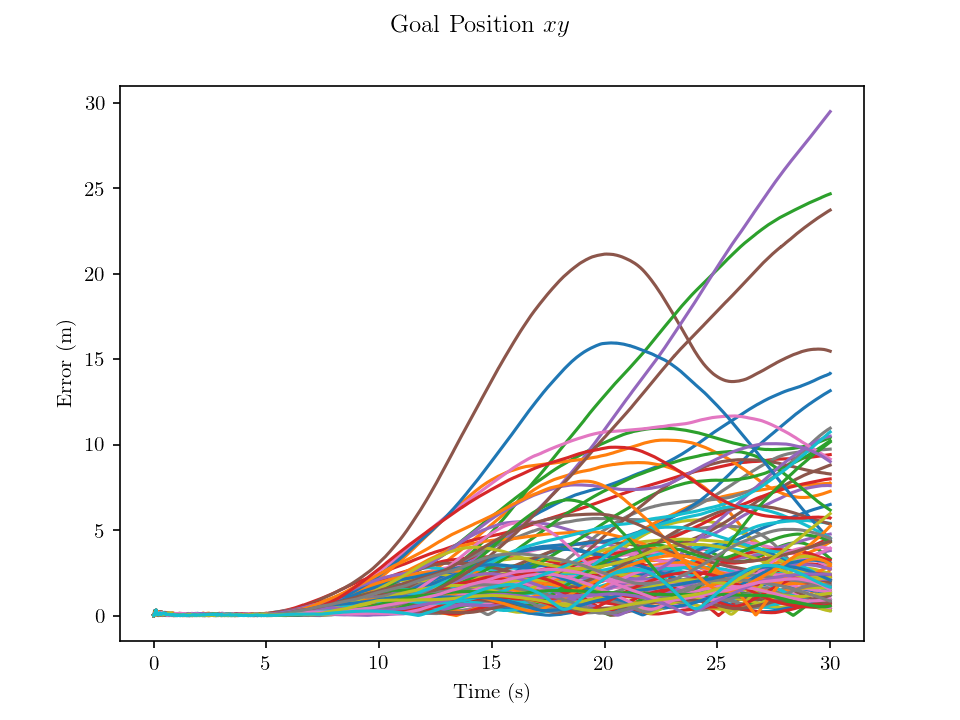
\includegraphics[scale=0.5]{plots/mc_no_lms_xy_err.png}
  \caption{Simulation results with estimator using no visual
  features. Measurements from the fiducial marker are not used after $t$ = 5
$s$ to demonstrate the performance of the estimator. The L2 norm of the error in
the x and y directions of the goal position is seen for 100 different simulation
runs.}
  \label{fig:mc_no_lms_xy_err}
\end{figure}

\begin{figure}
  \centering
  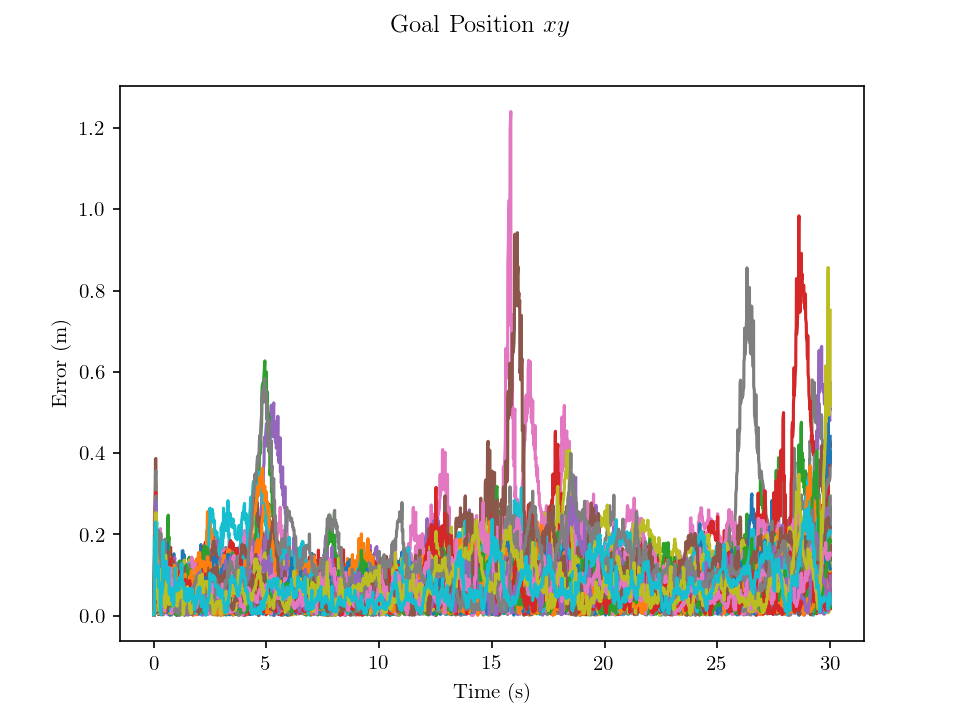
\includegraphics[scale=0.5]{plots/mc_with_lms_xy_err.png}
  \caption{Simulation results with estimator using a maximum of ten visual
  features. Measurements from the fiducial marker are not used after $t$ = 5
$s$ to demonstrate the performance of the estimator. The L2 norm of the error in
the x and y directions of the goal position is seen for 100 different simulation
runs.}
  \label{fig:mc_with_lms_xy_err}
\end{figure}

